\documentclass[10pt]{article}

\usepackage[margin=0.92in]{geometry}
\usepackage{fontspec}
\usepackage{kotex}
\setmainhangulfont{UnBatang.ttf}[
  BoldFont=UnBatangBold.ttf,
  ItalicFont=UnBatang.ttf,
  BoldItalicFont=UnBatangBold.ttf
]
\usepackage{setspace}
\usepackage{amsmath,amssymb,amsthm,mathtools}
\usepackage{booktabs}
\usepackage{graphicx}
\usepackage{caption}
\usepackage{subcaption}
\usepackage{algorithm}
\usepackage[noend]{algpseudocode}
\usepackage{enumitem}
\usepackage{xcolor}
\usepackage{natbib}
\usepackage{hyperref}
\usepackage[nameinlink,noabbrev]{cleveref}

\definecolor{linkblue}{RGB}{38,84,124}
\hypersetup{
  colorlinks=true,
  linkcolor=linkblue,
  citecolor=linkblue,
  urlcolor=linkblue,
  pdftitle={마스킹 이산 확산 언어 모델을 위한 측지 모멘텀 샘플링},
  pdfauthor={Yoonseong Jeong}
}

\graphicspath{{figures/}}
\setlist{nosep,leftmargin=1.5em}
\captionsetup{font=small,labelfont=bf}
\setstretch{1.075}
\setlength{\parskip}{0.18em}
\renewcommand{\abstractname}{초록}
\renewcommand{\refname}{참고문헌}
\renewcommand{\figurename}{그림}
\renewcommand{\tablename}{표}
\renewcommand{\proofname}{증명}

\theoremstyle{definition}
\newtheorem{proposition}{명제}
\newtheorem{corollary}{따름정리}
\newtheorem{remark}{비고}
\newtheorem{assumption}{가정}
\crefname{proposition}{명제}{명제}
\crefname{equation}{식}{식}
\crefname{table}{표}{표}
\crefname{figure}{그림}{그림}
\floatname{algorithm}{알고리즘}
\algrenewcommand\algorithmicrequire{\textbf{입력:}}
\algrenewcommand\algorithmicfor{\textbf{각각에 대해}}
\algrenewcommand\algorithmicdo{\textbf{반복}}
\algrenewcommand\algorithmicif{\textbf{만약}}
\algrenewcommand\algorithmicthen{\textbf{이면}}
\algrenewcommand\algorithmicelse{\textbf{아니면}}

\newcommand{\simplex}{\Delta^{V-1}}
\newcommand{\sphere}{\mathbb{S}^{V-1}}
\newcommand{\sphereplus}{\mathbb{S}^{V-1}_{+}}
\newcommand{\FR}{\mathrm{FR}}
\newcommand{\Exp}{\operatorname{Exp}}
\newcommand{\Log}{\operatorname{Log}}
\newcommand{\Slerp}{\operatorname{Slerp}}
\newcommand{\Projplus}{\operatorname{Proj}_{+}}
\newcommand{\Cat}{\operatorname{Cat}}
\newcommand{\mask}{\mathtt{m}}
\newcommand{\eps}{\varepsilon}

\title{\textbf{마스킹 이산 확산 언어 모델을 위한 측지 모멘텀 샘플링}\\
\large 추론 시점 Fisher--Rao 외삽법}
\author{Yoonseong Jeong\\KAIST 전산학부}
\date{검토용 번역 초안 --- 2026년 7월}

\begin{document}
\maketitle

\begin{abstract}
마스킹 이산 확산 언어 모델은 범주형 잡음 제거 전이를 연속적으로 수행하여 텍스트를 생성한다.
본 연구는 토큰별 범주형 예측을 Fisher--Rao 통계 다양체 위의 점으로 취급하는 추론 시점 수정법을
다룬다. 제곱근 사상은 범주형 단체를 초구의 양의 직교영역에 매장하며, 이 공간에서는 닫힌형식의
구면 보간을 사용할 수 있다. 각 역방향 단계에서 이전 외삽 예측에서 현재 모델 예측을 통과하는
대원의 호를 재귀적으로 연장하고, 그 결과를 다시 범주형 분포로 변환한 뒤 원래 MDLM 또는 SEDD
전이에 삽입한다. 이 방법을 \textbf{측지 모멘텀 샘플링}이라 부른다.

정확한 기하학적 유도를 제시하고, 사영 이전 갱신이 지수사상에 의한 연장과 동치임을 증명하며,
작은 각도에서의 계수가 가변 스텝 2단계 Adams--Bashforth 외삽 계수와 일치함을 보인다. 동시에
이 유사성의 한계를 분명히 한다. 본 방법은 접벡터장이 아니라 예측 분포를 외삽하고, 확률적 범주형
점프를 유지하며, 양의 직교영역으로의 사영을 사용한다. 따라서 이 방법은 2차 정확도의 확률흐름
ODE 솔버가 아니며, 2차 수렴성을 주장하지 않는다. OpenWebText 체크포인트로 수행되어 보존된
실험 결과는 MDLM의 10--100 역방향 스텝과 SEDD의 10--50 스텝에서 GPT-2 생성 퍼플렉서티가
개선될 가능성을 보여준다.
\end{abstract}

\section{서론}

이산 확산 언어 모델은 병렬적이고 양방향적인 생성을 제공하지만, 정확한 샘플링에는 흔히 많은
역방향 전이가 필요하다. MDLM은 치환 매개화를 통해 흡수 상태 확산을 단순화하고 효율적인 캐시
샘플러를 제공한다 \citep{sahoo2024mdlm}. 반면 SEDD는 구체적인 스코어 비율을 학습하고 해석적인
역방향 전이를 허용한다 \citep{lou2024sedd}. 두 모델은 모두 어휘집 위의 범주형 분포를 반복적으로
생성하는 방식으로 작동한다.

정보기하는 이러한 분포에 자연스러운 기하를 부여한다. 범주형 단체의 내부에는 Fisher--Rao 계량이
정의되며 \citep{amari2016information}, 제곱근 사상은 상수 배율을 제외하면 이를 구면의 양의
직교영역과 동일시한다. 이 구조는 Fisher-Flow \citep{davis2024fisherflow}와 연속 리만 확산 언어
모델(RDLM) \citep{jo2025rdlm}의 토대이기도 하다. 이들 방법은 구면 위의 연속 흐름을 학습하거나
시뮬레이션한다. 본 연구의 설정은 다르다. 사전학습된 이산 MDLM과 SEDD는 그대로 유지하고,
추론 시점의 범주형 예측만 수정한다.

본 연구의 주요 기여는 다음과 같다.
\begin{itemize}
  \item 정확한 제곱근 매장과 구면 선형 보간(SLERP)을 사용해 범주형 예측을 재귀적으로 측지
  외삽하는 방법을 정식화한다.
  \item 사영 이전 갱신이 지수사상에 의한 연장임을 보이고, 국소적인 Adams--Bashforth 유사 계수
  구조를 유도한다.
  \item 동일한 기하 연산자를 MDLM의 정답 토큰 예측과 SEDD의 해석적 전이 분포라는 서로 다른
  두 인터페이스에 적용한다.
  \item 불변량과 고차 방법과의 유사성이 성립하는 정확한 범위를 명시한다. 특히 본
  알고리즘을 RDLM 확률흐름 ODE 솔버와 동일시하지 않는다.
  \item 여섯 가지 역방향 스텝 수에서 MDLM 및 SEDD의 품질 결과를 보고한다.
\end{itemize}

\section{배경}

\subsection{범주형 Fisher--Rao 기하}

범주형 확률 단체를 다음과 같이 두자.
\begin{equation}
  \simplex
  = \left\{p\in\mathbb{R}^{V}: p_k\ge 0,\ \sum_{k=1}^{V}p_k=1\right\}.
\end{equation}
단체의 내부에서 접벡터는 $\sum_k v_k=0$을 만족하며, Fisher--Rao 계량은
\begin{equation}
  g_p(v,w)=\sum_{k=1}^{V}\frac{v_kw_k}{p_k}
  \label{eq:fisher_metric}
\end{equation}
이다.

\begin{proposition}[제곱근 등거리사상]
$\Psi:\operatorname{int}(\simplex)\rightarrow\sphereplus(2)$를 원소별 연산
$\Psi(p)=2\sqrt{p}$로 정의하자. 여기서 $\sphereplus(2)$는 반지름이 2인 구면의 양의
직교영역이다. 그러면 $\Psi$는 Fisher--Rao 계량과 주변 유클리드 공간이 유도하는 계량 사이의
등거리사상이다.
\end{proposition}

\begin{proof}
$\psi_k=2\sqrt{p_k}$이면 $d\psi_k=dp_k/\sqrt{p_k}$이므로
\begin{equation}
  \lVert d\psi\rVert_2^2
  =\sum_k\frac{dp_k^2}{p_k}
  =ds_{\FR}^2.
\end{equation}
또한 $\lVert\psi\rVert_2^2=4\sum_k p_k=4$이므로 $\psi$는 반지름 2인 구면 위에 놓인다.
\end{proof}

구현에서는 단위구면 좌표
\begin{equation}
  u(p)=\sqrt{p}\in\sphereplus
  \label{eq:sqrt_map}
\end{equation}
를 사용한다. 이는 상수 2배만큼만 차이가 난다.
$p,q\in\operatorname{int}(\simplex)$에 대해 두 점 사이의 구면각은
\begin{equation}
  \omega(p,q)
  =\arccos\langle u(p),u(q)\rangle
  =\arccos\left(\sum_k\sqrt{p_kq_k}\right)
  \label{eq:bhattacharyya_angle}
\end{equation}
이고, 반지름 2 관례에서의 Fisher--Rao 거리는 $d_{\FR}(p,q)=2\omega(p,q)$이다.
이 거리 공식은 닫힌 단체로 연속적으로 확장되어 그 거리 완비화를 정의하지만, 경계점 자체는
Fisher--Rao 리만 다양체의 매끄러운 점이 아니다.

\subsection{마스킹 이산 확산과 MDLM}

$\mask$을 흡수 마스크 상태, $\sigma(t)$를 적분 잡음 스케줄이라 하자. 시각 $t$까지 마스크로
이동했을 확률은
\begin{equation}
  m(t)=1-\exp[-\sigma(t)]
\end{equation}
이다. 역방향 스텝 $t>s$에서 MDLM은 정답 토큰 분포
$p_{\theta,t}(\cdot\mid x_t)$를 예측한다. 흡수 상태 매개화에서는
$p_{\theta,t}(\mask\mid x_t)=0$이고
$\sum_{k\ne\mask}p_{\theta,t}(k\mid x_t)=1$이다. $x_t=\mask$일 때 기준 구현은 다음 비정규화 가중치에서
표본을 추출한다.
\begin{equation}
  \widetilde q^{\mathrm{MDLM}}_{s\mid t}(k\mid x_t=\mask)=
  \begin{cases}
    [m(t)-m(s)]p_{\theta,t}(k\mid x_t), & k\neq\mask,\\
    m(s), & k=\mask.
  \end{cases}
  \label{eq:mdlm_transition}
\end{equation}
범주형 샘플링에서는 공통 정규화 상수가 중요하지 않다. $x_t\neq\mask$이면 흡수형 역방향
샘플러는 이미 마스크가 해제된 토큰을 그대로 복사한다. 캐시 샘플러는 이산 상태가 바뀔 때까지
$p_{\theta,t}$를 재사용한다 \citep{sahoo2024mdlm}.

\subsection{SEDD의 해석적 전이}

SEDD는 $p_t(y)/p_t(x)$를 근사하는 구체적 스코어 비율을 학습한다 \citep{lou2024sedd}.
$r_\theta(x_t,t)$를 학습된 스코어 벡터, $\mathcal{S}_{\Delta\sigma}$를 staggered-score 변환,
$K_{\Delta\sigma}(x_t,\cdot)$를 이동된 순방향 커널이라 하자. 해석적 샘플러는
\begin{equation}
  \widetilde q^{\mathrm{SEDD}}_{s\mid t}
  =\mathcal{S}_{\Delta\sigma}\!\left(r_\theta(x_t,t)\right)
   \odot K_{\Delta\sigma}(x_t,\cdot),
  \qquad
  \Delta\sigma=\sigma(t)-\sigma(s)
  \label{eq:sedd_transition}
\end{equation}
를 사용한 뒤 범주형 샘플링을 수행한다. 본 SEDD 변형은 스코어 벡터 자체가 아니라
\cref{eq:sedd_transition}을 정규화한 분포에 기하 연산을 적용한다.

\section{측지 모멘텀 샘플링}

\subsection{공통 분포 인터페이스}

각 배치 원소와 시퀀스 위치에 대해 역방향 인덱스 $i$에서의 범주형 분포
$z_i\in\simplex$를 다음과 같이 정의한다.
\begin{equation}
  z_i =
  \begin{cases}
    p_{\theta,t_i}(\cdot\mid x_{t_i}), & \text{MDLM},\\
    \operatorname{Normalize}(\widetilde q^{\mathrm{SEDD}}_{t_{i+1}\mid t_i}), & \text{SEDD}.
  \end{cases}
  \label{eq:common_distribution}
\end{equation}
원래 구면 좌표는 $u_i=\sqrt{z_i}$이다. $\widehat u_{i-1}$를 직전 단계에서 \textbf{외삽된}
좌표라 하자. 이 재귀적 선택은 중요하다. 즉, 본 방법은 최근 두 원시 예측만 보존하는 것이 아니라
지속적인 모멘텀을 갖는다.

\subsection{정확한 구면 연장}

단위벡터 $a,b\in\sphere$와 두 벡터 사이의 각
$\omega=\arccos\langle a,b\rangle\in(0,\pi)$에 대해 SLERP는 \citep{shoemake1985slerp}
\begin{equation}
  \Slerp(a,b;\tau)
  =\frac{\sin[(1-\tau)\omega]}{\sin\omega}a
   +\frac{\sin(\tau\omega)}{\sin\omega}b
  \label{eq:slerp}
\end{equation}
이다. 보간에는 $\tau\in[0,1]$을 사용하지만, 본 연구에서는 $\tau=1+\alpha_i$를 선택한다.
\begin{equation}
  e_i
  =\frac{\sin(-\alpha_i\omega_i)}{\sin\omega_i}\widehat u_{i-1}
   +\frac{\sin[(1+\alpha_i)\omega_i]}{\sin\omega_i}u_i,
  \quad
  \omega_i=\arccos\langle\widehat u_{i-1},u_i\rangle.
  \label{eq:geodesic_extrapolation}
\end{equation}

\begin{proposition}[지수사상 표현]
서로 다르고 대척점도 아닌 $a,b\in\sphere$와 $\alpha\ge 0$에 대해
\begin{equation}
  \Slerp(a,b;1+\alpha)
  =\Exp_b\!\left[-\alpha\Log_b(a)\right]
  \label{eq:exp_equivalence}
\end{equation}
가 성립한다. 따라서 \cref{eq:geodesic_extrapolation}은 아래에서 설명할 양수화 연산을 적용하기
전에 $a$에서 출발해 $b$를 지나는 대원의 호를 추가 비율 $\alpha$만큼 정확히 연장한다.
\end{proposition}

\begin{proof}
$\gamma(\tau)=\Slerp(a,b;\tau)$는 $\tau\in[0,1]$에서 $a$와 $b$를 연결하는 유일한 최단 대원
구간이다. $b=\gamma(1)$에서 $-\Log_b(a)$는 노름이 $\omega$인 순방향 연장 접벡터다.
크기가 조절된 벡터 $-\alpha\Log_b(a)$에 $\Exp_b$를 적용하면 호의 길이 $\alpha\omega$만큼
전진하므로, 이는 정확히 $\gamma(1+\alpha)$와 같다.
\end{proof}

$a=b$, 즉 $\omega=0$일 때는 연속 확장으로 $\Slerp(a,a;\tau)=a$라 정의하며, 이 경우에도
명제는 성립한다. \cref{eq:slerp,eq:exp_equivalence}은 클램프하지 않은 이상적 연산자를
기술한다. 구현은 수치 안정성을 위해 각도를 다음과 같이 계산한다.
\[
\arccos\!\bigl(\operatorname{clamp}(\langle a,b\rangle,-1+\eps,1-\eps)\bigr).
\]
따라서 정확한
지수사상 항등식은 이상적 연산자에 대한 것이며, 실제 구현은 끝점 부근에서 안정화한 근사다.

\subsection{양의 직교영역 사영과 확률 복원}

대원을 따른 외삽은 양의 직교영역을 벗어날 수 있다. 보존된 구현은
\begin{equation}
  \Projplus(e)=\frac{[e]_+}{\lVert[e]_+\rVert_2},
  \qquad [e]_{+,k}=\max(e_k,0)
  \label{eq:retraction}
\end{equation}
를 사용하고, 다음과 같이 확률을 복원한다.
\begin{equation}
  \widehat z_{i,k}=(\widehat u_{i,k})^2,
  \qquad \widehat u_i=\Projplus(e_i).
  \label{eq:prob_recovery}
\end{equation}

\begin{proposition}[확률의 유효성]
$\lVert[e_i]_+\rVert_2>0$이면 복원된 벡터 $\widehat z_i$는 $\simplex$에 속한다.
\end{proposition}

\begin{proof}
각 성분은 제곱이므로 음수가 아니다. 또한 $\widehat u_i$의 노름이 1이므로
$\sum_k\widehat z_{i,k}=\sum_k\widehat u_{i,k}^2=1$이다.
\end{proof}

이 사영은 실용적인 영역 보정이며, 정확한 Fisher--Rao 측지선의 일부가 아니다. 성분이 0을
가로지르는 곳에서 매끄럽지 않고 $[e]_+=0$이면 정의되지 않으므로, 고차 측지 적분기의 보장을
직접 계승할 수 없다.

\subsection{스텝 계수와 AB2 유사성}

감소하는 역방향 격자를 $t_0>t_1>\cdots>t_N$이라 하고, 양의 스텝 크기를
$h_i=t_i-t_{i+1}$로 정의하자. 구현에서는
\begin{equation}
  \alpha_i=c_i\frac{h_i}{2h_{i-1}},\qquad \alpha_0=0
  \label{eq:alpha}
\end{equation}
을 사용한다. 보존된 SEDD 실행에서는 $c_i=1$이고, MDLM에서는
\begin{equation}
  c_i=c\min\left(1,\frac{h_i}{h_{\mathrm{ref}}}\right),
  \qquad c=1,\quad h_{\mathrm{ref}}=\frac{1}{50}
  \label{eq:dynamic_damping}
\end{equation}
을 사용한다.

\begin{proposition}[국소 선형 형태]
고정된 $\alpha$와 $\omega=\arccos\langle a,b\rangle\rightarrow0$에 대해
\begin{equation}
  \Slerp(a,b;1+\alpha)
  =(1+\alpha)b-\alpha a+O(\omega^2)
  \label{eq:local_linear}
\end{equation}
가 성립한다. $c_i=1$이고 $r_i=h_i/h_{i-1}$이면 선도 계수는
$(1+r_i/2,-r_i/2)$이며, 이는 가변 스텝 AB2의 계수와 일치한다.
\end{proposition}

\begin{proof}
\cref{eq:slerp}에서 $\tau=1+\alpha$로 두고
$\sin(\beta\omega)/\sin\omega=\beta+O(\omega^2)$를 사용하면
$\sin(-\alpha\omega)/\sin\omega=-\alpha+O(\omega^2)$ 및
$\sin[(1+\alpha)\omega]/\sin\omega=1+\alpha+O(\omega^2)$를 얻는다.
\end{proof}

\begin{remark}[리만 AB2가 아닌 이유]
리만 AB2는 $V_{i-1}$을 $T_{X_i}\mathcal{M}$으로 평행이동한 뒤 접공간의 벡터장
$V_i\in T_{X_i}\mathcal{M}$과 결합하고, 지수사상으로 상태를 갱신한다
\citep{hairer2006geometric}. 반면 \cref{eq:local_linear}은 \textbf{범주형 예측을 나타내는 점}을
결합할 뿐이며 접벡터장을 평가하거나 평행이동하지 않는다. 따라서 계수의 일치는 국소적인 유사성일
뿐, 정확도 차수에 대한 증명이 아니다.
\end{remark}

\subsection{MDLM 및 SEDD에 대한 구체화}

MDLM에서는 $\widehat z_i$가 \cref{eq:mdlm_transition}의 $p_{\theta,t_i}$를 대체하며, 이미
마스크가 해제된 토큰은 고정된다. SEDD에서는 $\widehat z_i$가 \cref{eq:sedd_transition}의
정규화된 해석적 전이를 직접 대체한다. 두 경우 모두 다음 토큰 상태는 Gumbel-max로 추출하므로,
모든 신경망 입력은 이산 상태로 유지된다.

\begin{algorithm}[t]
\caption{MDLM 또는 SEDD를 위한 측지 모멘텀 샘플링}
\label{alg:gms}
\begin{algorithmic}[1]
\Require 사전학습 모델, 역방향 격자 $t_0>\cdots>t_N$, 모드 $\in\{\mathrm{MDLM},\mathrm{SEDD}\}$
\State $x\gets$ 전체 마스크 사전분포; $\widehat u_{-1}\gets\varnothing$
\For{$i=0,\ldots,N-1$}
  \If{모드가 MDLM이면}
    \State $z_i\gets p_{\theta,t_i}(\cdot\mid x)$
  \Else
    \State \cref{eq:sedd_transition}으로 $\widetilde q_i$ 구성;
    $z_i\gets\operatorname{Normalize}(\widetilde q_i)$
  \EndIf
  \State $u_i\gets\sqrt{z_i}$; \cref{eq:alpha}로 $\alpha_i$ 계산
  \If{$i=0$}
    \State $\widehat u_i\gets u_i$
  \Else
    \State $e_i\gets\Slerp(\widehat u_{i-1},u_i;1+\alpha_i)$
    \State $\widehat u_i\gets\Projplus(e_i)$
  \EndIf
  \State $\widehat z_i\gets\widehat u_i^{\odot2}$
  \If{모드가 MDLM이면}
    \State $\widehat z_i$를 \cref{eq:mdlm_transition}에 삽입; 마스크 위치를 샘플링하고 나머지는 복사
  \Else
    \State $x\sim\Cat(\widehat z_i)$
  \EndIf
\EndFor
\State 기준 방법의 마지막 잡음 제거 단계를 적용하고 $x$ 반환
\end{algorithmic}
\end{algorithm}

\section{이론적 적용 범위와 주장하지 않는 사항}

본 방법은 다음의 정확한 성질을 보존한다.
\begin{enumerate}
  \item \textbf{이산 상태 호환성.} 모델은 항상 정수 토큰 인덱스를 입력받는다.
  \item \textbf{첫 스텝의 동치성.} $\alpha_0=0$이므로 같은 난수 추출을 사용할 때 첫 범주형 전이는
  대응하는 기준 전이와 동일하다.
  \item \textbf{단체 유효성.} 사영할 양의 부분이 0이 아니라는 조건 아래 모든 외삽 분포는 음이 아닌
  값으로 정규화된다.
  \item \textbf{MDLM 흡수 구조.} 이미 마스크가 해제된 토큰은 캐시를 사용하지 않는 MDLM 역방향
  전이와 정확히 동일하게 고정된다.
\end{enumerate}

그러나 샘플 시퀀스 $x_{t_i}$는 확률적으로 변하므로 $z_i$는 결정론적 주변분포 곡선 $p_t$가 아니라
무작위 경로를 따라 얻은 조건부 예측들의 모음이다. SEDD에서 $z_i$는 확률흐름 ODE의 상태가 아니라
한 스텝 전이 분포다. 또한 $p_k=0$인 경계에서 Fisher--Rao 계량은 특이하지만, MDLM은 의도적으로
마스크 확률을 0으로 설정하고 이미 마스크가 해제된 토큰에는 델타 분포를 만든다. 제곱근 표현은 이
경계에서도 수치적으로 사용할 수 있으나, 매끄러운 다양체에 기반한 Taylor 가정은 성립하지 않는다.

RDLM은 초구 위에 연속적인 브리지 혼합 SDE를 구성하고 연속 상태를 조건으로 하는 모델을 학습한다
\citep{jo2025rdlm}. Fisher-Flow는 구면 측지선을 따라 확률질량을 운반하는 연속 벡터장을 학습한다
\citep{davis2024fisherflow}. 본 방법은 이 두 작업을 수행하지 않는다. 마찬가지로 DPM-Solver는
확산 ODE의 정확한 준선형 적분 형태를 활용하여 고차 정확도를 얻지만 \citep{lu2022dpmsolver}, 현재
이산 샘플러에는 그와 같은 구조가 없다. 따라서 본 연구는 주변분포 보존, 국소 절단오차 $O(h^3)$,
또는 전역 수렴 $O(h^2)$를 주장하지 않는다.

\section{실험 결과의 평가}

\subsection{프로토콜}

실험 스크립트는 MDLM을 자체 \texttt{ddpm\_cache} 샘플러와 비교하고, SEDD를 자체 해석적
샘플러와 비교한다. 두 실험 모두 MDLM 코드베이스의 OpenWebText 체크포인트와 시퀀스 길이 1024를
사용한다. 역방향 스텝 수는 $10$, $20$, $50$, $100$, $256$, $512$이다. 품질 지표는 다음과 같다.
\begin{itemize}
  \item GPT-2로 계산한 토큰 가중 퍼플렉서티. 낮을수록 좋다.
  \item 생성 텍스트와 참조 텍스트의 유니그램 토큰 히스토그램 사이의 Jensen--Shannon 발산.
  낮을수록 좋다. 참조 문장은 WikiText-2 원시 검증 부분집합에서 가져온 비어 있지 않은 문자열이다.
\end{itemize}

\subsection{품질 결과}

\begin{table}[t]
\centering
\small
\caption{품질 결과. $\mathrm{Gain}_{\mathrm{PPL}}
=100(\mathrm{baseline}-\mathrm{geodesic})/\mathrm{baseline}$이며, 양수이면 측지 모멘텀이
우세하다. 굵은 글씨는 각 쌍에서 더 낮은 값을 나타낸다.}
\label{tab:quality}
\begin{tabular}{llrrrrr}
\toprule
모델 & 스텝 & 기준 PPL & 측지 PPL & $\mathrm{Gain}_{\mathrm{PPL}}$ & 기준 JS & 측지 JS \\
\midrule
MDLM & 10  & 551.953 & \textbf{407.473} & $+26.18\%$ & \textbf{0.38659} & 0.38850 \\
     & 20  & 261.453 & \textbf{212.993} & $+18.53\%$ & \textbf{0.37718} & 0.38073 \\
     & 50  & 140.075 & \textbf{120.542} & $+13.95\%$ & \textbf{0.36864} & 0.37629 \\
     & 100 & 92.421  & \textbf{81.864}  & $+11.42\%$ & 0.38260 & \textbf{0.38185} \\
     & 256 & \textbf{65.431} & 65.665 & $-0.36\%$ & \textbf{0.37828} & 0.38066 \\
     & 512 & \textbf{50.905} & 51.801 & $-1.76\%$ & 0.38224 & \textbf{0.37800} \\
\midrule
SEDD & 10  & 486.276 & \textbf{434.932} & $+10.56\%$ & \textbf{0.35628} & 0.36043 \\
     & 20  & 235.867 & \textbf{214.863} & $+8.91\%$  & 0.34810 & \textbf{0.34707} \\
     & 50  & 123.169 & \textbf{114.949} & $+6.67\%$  & 0.34771 & \textbf{0.34503} \\
     & 100 & \textbf{82.088} & 84.184 & $-2.55\%$ & 0.35678 & \textbf{0.35078} \\
     & 256 & \textbf{59.954} & 63.276 & $-5.54\%$ & \textbf{0.34519} & 0.34670 \\
     & 512 & 51.695 & \textbf{50.903} & $+1.53\%$ & \textbf{0.36408} & 0.36661 \\
\bottomrule
\end{tabular}
\end{table}

\begin{figure}[t]
  \centering
  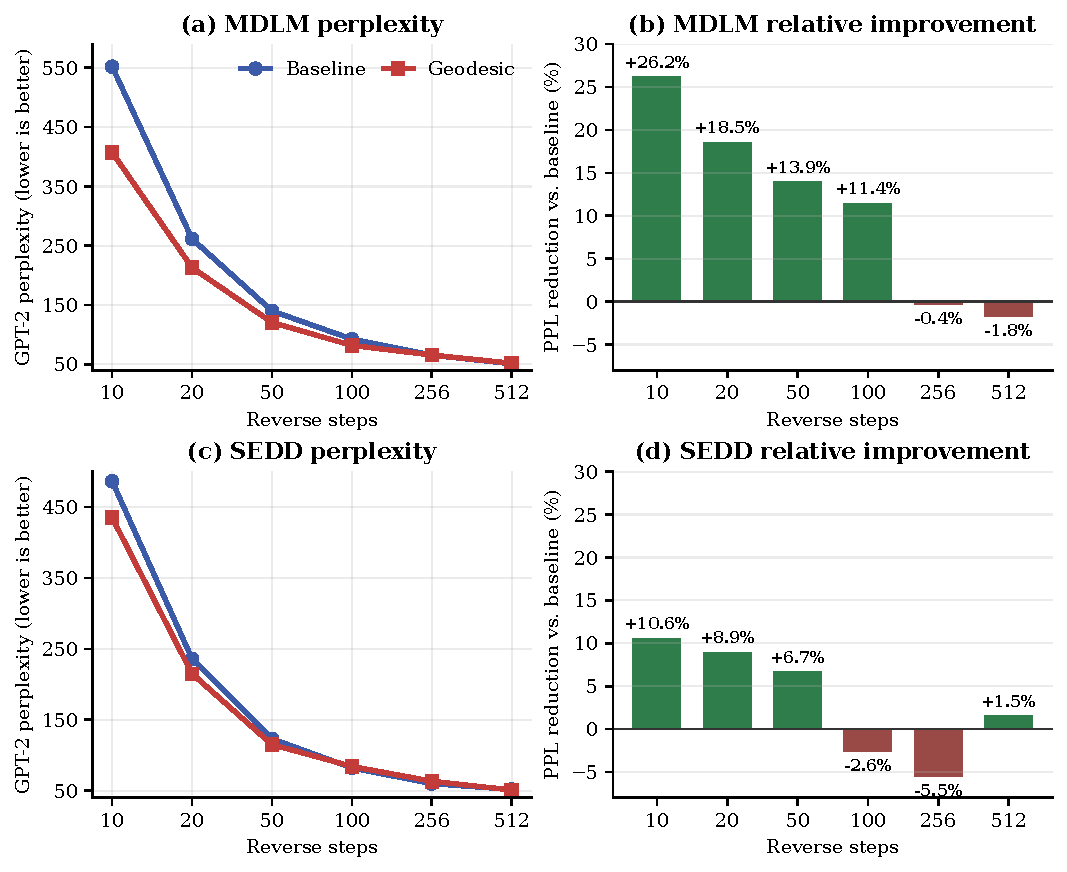
\includegraphics[width=0.94\linewidth]{quality_curves.pdf}
  \caption{퍼플렉서티 결과. 왼쪽 패널은 각 모델의 관측 범위에 맞춘 선형 세로축으로 원시
  GPT-2 퍼플렉서티를 표시하므로 적은 스텝에서의 차이를 직접 확인할 수 있다. 오른쪽 패널은
  상대 PPL 감소율 $(\mathrm{baseline}-\mathrm{geodesic})/\mathrm{baseline}$을 나타낸다.
  양의 막대는 개선, 음의 막대는 저하를 뜻한다. 두 개선률 패널은 같은 $[-8,30]$ 퍼센트포인트
  범위를 유지한다.}
  \label{fig:quality_curves}
\end{figure}

MDLM의 10, 20, 50, 100 스텝에서 측지 샘플의 GPT-2 퍼플렉서티는 각각 26.18\%,
18.53\%, 13.95\%, 11.42\% 낮다. 256 및 512 스텝에서는 차이가 사라지고 기준 방법이 약간
우세하다. 이 패턴은 적은 스텝을 보정하려는 본 방법의 의도와 일치한다.
\cref{eq:dynamic_damping}의 MDLM 감쇠는 균일 격자의
스텝 수가 50을 넘으면 $\alpha$도 감소시킨다. 그 값은 100, 256, 512 스텝에서 각각 약
$0.25$, $0.098$, $0.049$다.

SEDD는 10--50 스텝에서 더 작은 퍼플렉서티 감소를 보이고, 100--256 스텝에서는 성능이
저하되며, 512 스텝에서는 작게 개선된다. 구현은 모든 균일 격자에서 첫 스텝 이후
$\alpha=1/2$을 사용했고 MDLM의 고스텝 감쇠는 사용하지 않았다. 이것이 오버슈트에 기여했을
가능성은 있으나, 현재 실험만으로 원인을 분리할 수는 없다. Jensen--Shannon 발산은 두 모델
모두에서 결과가 혼재하며 일관된 분포 개선을 보이지 않는다.

\section{논의}

\paragraph{해석.}
가장 방어 가능한 해석은 예측 지연 보정이다. 역방향 스텝이 적으면 연속된 잡음 제거 분포 또는
전이 분포가 크게 이동할 수 있다. 최근 Fisher--Rao 호를 연장하면 다음 예측을 앞서 추정하여 품질을
개선할 수 있다. 격자가 촘촘해질수록 원시 예측의 변화가 작아지므로 외삽의 이점은 줄어들고,
확률적 오차나 모델 오차를 증폭할 수 있다.

\paragraph{MDLM과 SEDD의 차이.}
MDLM은 흡수 전이 이전의 정답 토큰 예측에 모멘텀을 적용하고 완료된 토큰을 고정한다. SEDD는
확률적 상태에 의존하는 한 스텝 전이에 모멘텀을 적용한다. 후자의 대상은 시간에 따라 덜 매끄러울 수
있으며, 이는 곡선 외삽이라는 해석을 약화시키고 보존된 결과의 불안정한 경향과도 일치한다.

\paragraph{연속 기하 모델과의 관계.}
본 방법은 Fisher-Flow 및 RDLM과 동일한 Fisher--Rao 매장을 사용하지만, 그 동역학을 사용하지는
않는다. 진정한 리만 다단계 솔버에는 연속 상태 $X_t$, 잘 정의된 접벡터장, $T_{X_{i-1}}\mathcal{M}$과
$T_{X_i}\mathcal{M}$ 사이의 평행이동, 그리고 지수사상에 의한 상태 갱신이 필요하다. 사전학습된
이산 MDLM 또는 SEDD를 위해 그러한 솔버를 확립하려면 범주형 예측과 연속 벡터장을 연결하는 새로운
유도가 필요하다.

\section{한계}

\begin{enumerate}
  \item \textbf{수렴 차수를 보장하지 않음.} 확률적 점프, 벡터가 아닌 점의 외삽, 재귀적 이력,
  매끄럽지 않은 사영 때문에 AB2의 차수 논증을 직접 적용할 수 없다.
  \item \textbf{경계 기하.} 정확히 0인 성분은 Fisher--Rao 계량이 특이해지는 경계에 예측을 놓는다.
  \item \textbf{위치별 근사.} 각 토큰 위치를 서로 분리된 범주형 단체로 취급한다. 전체 결합 시퀀스
  분포의 기하는 표현하지 않는다.
\end{enumerate}

\section{결론}

본 논문은 Fisher--Rao 제곱근 구면 위에서 범주형 예측을 재귀적으로 외삽하는 MDLM 및 SEDD의
추론 시점 수정법인 측지 모멘텀 샘플링을 제시했다. 양의 직교영역 사영 이전의 갱신은 정확한
지수사상 해석을 가지며, 국소 계수는 가변 스텝 AB2 계수와 일치한다. 그러나 이 알고리즘은
확률흐름 ODE의 평행이동된 벡터장이 아니라 확률적 이산 경로에서 얻은 예측 점에 작용한다. 따라서
수학적으로 정확한 명칭은 증명된 2차 리만 솔버가 아니라 \textbf{재귀적 Fisher--Rao 구면 외삽}이다.

결과는 특히 MDLM의 적은 스텝에서 유망한 퍼플렉서티 경향을 보이지만, 분포 지표와 SEDD의
고스텝 결과는 혼재한다. 형식적인 수렴성을 주장하려면 연속 벡터장에 기반한 유도가 필요하다.


\bibliographystyle{plainnat}
\bibliography{references}

\end{document}
